\section{Riemann问题}
\label{sec:cons-riemann}

最简单的不连续初值是左右两个常状态：
\begin{equation}
  u_0(x)=\begin{cases}u_l,&x<0,\\u_r,&x>0.\end{cases}
  \label{eq:cons-riemann-data}
\end{equation}
这称为\term{Riemann问题}（Riemann problem）。守恒、特征线和熵条件在这里都能落实成手算。

有一条结构可以先用上。方程和初值在缩放$(x,t)\mapsto(\lambda x,\lambda t)$下不变，若解唯一（下一节证明），解就只依赖于比值$\xi=x/t$，形如$u=w(\xi)$。这样的解称为\term{自相似解}（self-similar solution）。在$(x,t)$平面上，它沿着从原点出发的每条射线取常值。

本节先设$F$严格凸。此时$F'$严格递增，按上一节的结论，$u_l>u_r$时阶跃本身是可接受的间断，$u_l<u_r$时不是。这两种情形分别对应两种完全不同的波。

\subsection{激波}
\label{subsec:cons-shock}

左状态大于右状态时，$F'(u_l)>F'(u_r)$，左边的特征线比右边的快，迎面相撞，只能产生间断。

\begin{theorem}[激波解]
\label{thm:cons-shock}
设$F\in C^1$严格凸，$u_l>u_r$。令
\begin{equation}
  s=\frac{F(u_l)-F(u_r)}{u_l-u_r},\qquad
  u(x,t)=\begin{cases}u_l,&x<st,\\u_r,&x>st.\end{cases}
  \label{eq:cons-shock-solution}
\end{equation}
则$u$是Riemann问题的熵解。
\end{theorem}

\begin{proof}
$u$分块为常数，满足方程。$s$由式~\eqref{eq:cons-shock-speed}给出，跳跃条件成立。由定理~\ref{thm:cons-chord}，$u_->u_+$时式~\eqref{eq:cons-jump-entropy}对所有凸熵对成立，所以式~\eqref{eq:cons-entropy-ineq}成立。最后，$u$与初值只在宽度为$\lvert s\rvert t$的区间上不同，差不超过$u_l-u_r$，式~\eqref{eq:cons-entropy-initial}成立。
\end{proof}

波速由两侧状态共同决定，任何一侧单独都定不下来。表~\ref{tab:cons-shock-examples}列出几组数据。Burgers方程的波速是两侧状态的算术平均，这是平方通量的特殊之处；最后一行的通量$F=u^4/4$严格凸，波速$15/4$并不等于两侧传播速度的平均$9/2$。每一行都满足$F'(u_l)>s>F'(u_r)$。

\begin{BookInlineTable}
  \centering
  \caption{激波速度的手算。前四行是Burgers方程，第五行$F=u^4/4$，每一行都验证了$F'(u_l)>s>F'(u_r)$。}
  \label{tab:cons-shock-examples}
  \begin{tabular}{cccccc}
    \toprule
    通量 & $u_l$ & $u_r$ & $s$ & $F'(u_l)$ & $F'(u_r)$\\
    \midrule
    $u^2/2$ & $2$ & $0$ & $1$ & $2$ & $0$\\
    $u^2/2$ & $2$ & $1$ & $3/2$ & $2$ & $1$\\
    $u^2/2$ & $1$ & $-1$ & $0$ & $1$ & $-1$\\
    $u^2/2$ & $0$ & $-2$ & $-1$ & $0$ & $-2$\\
    $u^4/4$ & $2$ & $1$ & $15/4$ & $8$ & $1$\\
    \bottomrule
  \end{tabular}
\end{BookInlineTable}

取第一行$u_l=2$、$u_r=0$，$s=1$，解在图~\ref{fig:cons-riemann-shock}中。用矩形$[-1,3]\times[0,1]$核对收支：初始总量是$2\cdot1=2$，$t=1$时$x<1$的部分长度为$2$，总量是$4$，左端流入$F(2)\cdot1=2$，右端流出$0$，正好$2+2=4$。第三行的$s=0$说明波速可以为零，第四行的$s=-1$说明激波可以向左传播。

\begin{BookInlineFigure}
  \centering
  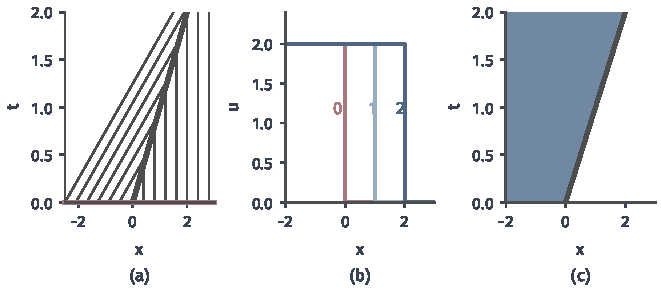
\includegraphics[width=112mm]{figures/06-differential-equations/02-partial-differential-equations/matplotlib/cons-riemann-shock/figure.pdf}
  \caption{Burgers方程的Riemann问题$u_l=2$、$u_r=0$，$s=1$。(a)特征线（细线）从两侧汇入激波（深灰粗线）。(b)红线是$t=0$，蓝色由浅到深是$t=1,2$。(c)时空平面上的场，颜色越深值越大。}
  \label{fig:cons-riemann-shock}
\end{BookInlineFigure}

\subsection{稀疏波}
\label{subsec:cons-rarefaction}

左状态小于右状态时，$F'(u_l)<F'(u_r)$，左边的特征线比右边的慢，它们彼此分开。图~\ref{fig:cons-riemann-fan}(a)中，浅红的楔形区域没有任何特征线到达，式~\eqref{eq:cons-implicit}在那里什么也没有告诉我们。阶跃本身还是可以当作弱解，但它在上一节已经被熵条件排除，楔形必须用别的东西填满。

\begin{BookInlineFigure}
  \centering
  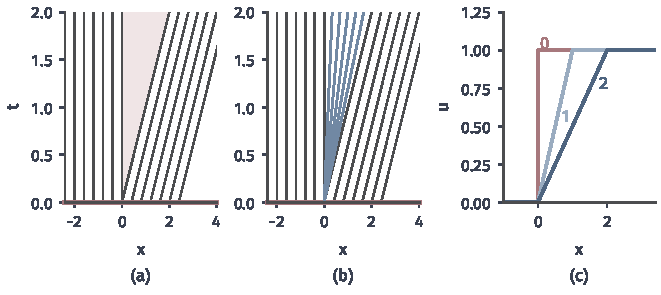
\includegraphics[width=112mm]{figures/06-differential-equations/02-partial-differential-equations/matplotlib/cons-riemann-fan/figure.pdf}
  \caption{Burgers方程的Riemann问题$u_l=0$、$u_r=1$。(a)只画初始线出发的特征线，留下一片浅红的空白楔形。(b)从原点发出的扇形特征线（蓝）填满楔形。(c)红线是$t=0$，蓝色由浅到深是$t=1,2$，斜坡的宽度随时间线性增长。}
  \label{fig:cons-riemann-fan}
\end{BookInlineFigure}

用自相似的形式求解。把$u=w(\xi)$，$\xi=x/t$代入式~\eqref{eq:cons-quasilinear}，$\partial_tu=-\xi w'/t$，$\partial_xu=w'/t$，得到
\[
  \frac{w'(\xi)}{t}\bigl(F'(w(\xi))-\xi\bigr)=0 .
\]

所以每一点要么$w'=0$（常状态），要么$F'(w(\xi))=\xi$。后者说明，填补楔形的解满足$F'(w)=\xi$，也就是把初始间断点看成同时发出所有速度的特征线的源头：每条射线$x=\xi t$就是一条特征线，速度恰好是$\xi$。这样得到的解称为\term{稀疏波}（rarefaction wave）。

\begin{theorem}[稀疏波解]
\label{thm:cons-rarefaction}
设$F\in C^2$，在$[u_l,u_r]$上$F''>0$，$u_l<u_r$。令
\begin{equation}
  u(x,t)=\begin{cases}
    u_l,&x\leq F'(u_l)\,t,\\
    (F')^{-1}(x/t),&F'(u_l)\,t<x<F'(u_r)\,t,\\
    u_r,&x\geq F'(u_r)\,t.
  \end{cases}
  \label{eq:cons-rarefaction}
\end{equation}
则$u$连续（$t>0$），并且是Riemann问题的熵解。
\end{theorem}

\begin{proof}
$F'$在$[u_l,u_r]$上严格递增，逆函数$(F')^{-1}$是$C^1$的，所以式~\eqref{eq:cons-rarefaction}有定义。在扇形边界上它的值分别是$u_l$、$u_r$，$u$在$t>0$连续。

在扇形内，记$w=(F')^{-1}$，有$F''(w)\,w'=1$，于是
\[
  \partial_tu+F'(u)\,\partial_xu
  =-\frac{x}{t^2}w'+\frac{x}{t}\cdot\frac{w'}{t}=0 .
\]

$u$在各块上是$C^1$的，满足方程，由链式法则，每一块上$\partial_t\eta(u)+\partial_xq(u)=0$。两条接缝上$u$连续，式~\eqref{eq:cons-jump-entropy}的左端为零。所以式~\eqref{eq:cons-entropy-ineq}取等号成立。最后，$u$只在宽度不超过$\max\lvert F'\rvert\,t$的区间上与初值不同，差不超过$u_r-u_l$，式~\eqref{eq:cons-entropy-initial}成立。
\end{proof}

Burgers方程$F'(u)=u$，$(F')^{-1}$是恒等映射，取$(u_l,u_r)=(0,1)$，得到
\begin{equation}
  u(x,t)=\frac{x}{t},\qquad 0<x<t,
  \label{eq:cons-burgers-fan}
\end{equation}
这正是前面的$u^{\mathrm{f}}$。$F=u^4/4$、$(u_l,u_r)=(1,2)$时，$F'(u)=u^3$，扇形占据$1<x/t<8$，解是$u=(x/t)^{1/3}$。扇形边缘的速度由两侧状态各自决定，而不是取什么平均：左边缘$F'(u_l)$，右边缘$F'(u_r)$。

\paragraph{扇形是连续依赖的结果}
稀疏波可以由经典解的极限得到。把阶跃$0$、$1$替换成宽度为$\varepsilon$的斜坡，$u_0=x/\varepsilon$（$0\leq x\leq\varepsilon$）。这个初值单调不减，定理~\ref{thm:cons-lifespan}说解永远不会失去光滑性。由特征线$x=x_0+(x_0/\varepsilon)t$反解$x_0=\varepsilon x/(\varepsilon+t)$，得到
\begin{equation}
  u^{\varepsilon}(x,t)=\frac{x}{\varepsilon+t},\qquad 0\leq x\leq\varepsilon+t .
  \label{eq:cons-smoothed-step}
\end{equation}

令$\varepsilon\to0$，式~\eqref{eq:cons-smoothed-step}收敛到扇形~\eqref{eq:cons-burgers-fan}，如图~\ref{fig:cons-smoothed-step}。所以向上的阶跃是一个不稳定的状态：无论把初值磨得多么轻微，解都立刻选择扇形。跳跃解$u^{\mathrm{j}}$经不起这样的扰动，这是排除它的又一条理由。

\begin{BookInlineFigure}
  \centering
  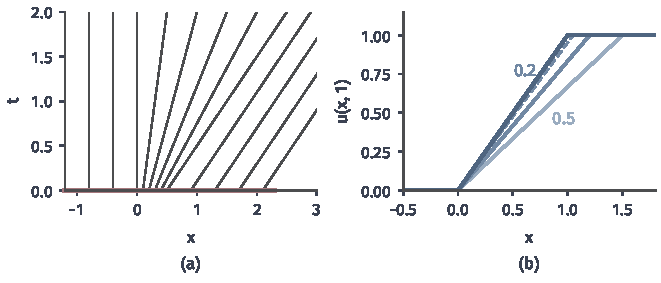
\includegraphics[width=112mm]{figures/06-differential-equations/02-partial-differential-equations/matplotlib/cons-smoothed-step/figure.pdf}
  \caption{磨光的阶跃。(a)$\varepsilon=0.5$的特征线，从斜坡出发的特征线彼此张开，永不相交。(b)解~\eqref{eq:cons-smoothed-step}在$t=1$的形状，蓝色由浅到深是$\varepsilon=0.5,0.2$，虚线是$\varepsilon=0.05$，最深的蓝线是扇形。}
  \label{fig:cons-smoothed-step}
\end{BookInlineFigure}

表~\ref{tab:cons-wave-comparison}把三种候选放在一起对比。

\begin{BookInlineTable}
  \centering
  \caption{严格凸通量下的三种波。}
  \label{tab:cons-wave-comparison}
  \begin{tabular}{cccc}
    \toprule
    & 激波 & 稀疏波 & 扩张间断\\
    \midrule
    状态 & $u_l>u_r$ & $u_l<u_r$ & $u_l<u_r$\\
    连续性 & 跳跃 & 连续 & 跳跃\\
    特征线 & 汇入 & 张开并填满 & 从间断发出\\
    能量（Burgers） & 减少 & 守恒 & 增加\\
    熵条件 & 满足 & 满足 & 违反\\
    \bottomrule
  \end{tabular}
\end{BookInlineTable}

\paragraph{波的相遇：方波}
Riemann解可以拼起来，用来算一般的初值。取Burgers方程和方波
\[
  u_0(x)=\begin{cases}1,&0<x<1,\\0,&\text{其他}.\end{cases}
\]

$x=0$处是向上的阶跃，产生扇形$u=x/t$；$x=1$处是向下的阶跃，产生激波，速度$1/2$。所以$t\leq2$时
\[
  u(x,t)=\begin{cases}x/t,&0<x<t,\\1,&t<x<1+t/2,\\0,&\text{其他}.\end{cases}
\]

扇形的右边缘$x=t$追赶激波$x=1+t/2$，相遇于$t=2$、$x=2$。此后激波左侧的状态不再是常数，而是扇形的值$\gamma/t$，右侧仍是$0$。由式~\eqref{eq:cons-burgers-speed}，激波位置$\gamma(t)$满足
\[
  \gamma'(t)=\frac{\gamma(t)}{2t},\qquad \gamma(2)=2 .
\]

分离变量解得$\gamma(t)=\sqrt{2t}$。于是$t\geq2$时的解是
\begin{equation}
  u(x,t)=\begin{cases}x/t,&0<x<\sqrt{2t},\\0,&\text{其他}.\end{cases}
  \label{eq:cons-box-late}
\end{equation}

波形成为一个三角形，高度$\gamma/t=\sqrt{2/t}$按$t^{-1/2}$衰减，底宽$\sqrt{2t}$按$t^{1/2}$增长。面积是
\[
  \frac12\cdot\sqrt{2t}\cdot\sqrt{\frac2t}=1 ,
\]
与初值的总量一致。图~\ref{fig:cons-box-interaction}展示了这个过程。

\begin{BookInlineFigure}
  \centering
  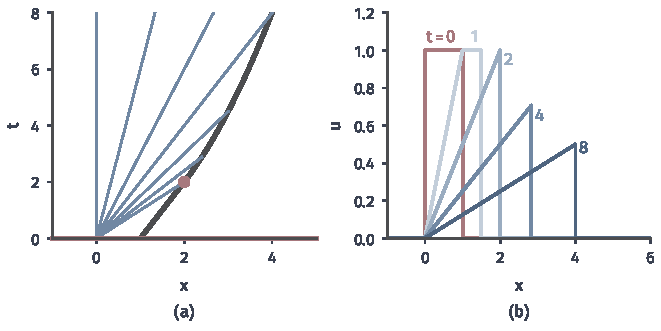
\includegraphics[width=112mm]{figures/06-differential-equations/02-partial-differential-equations/matplotlib/cons-box-interaction/figure.pdf}
  \caption{方波的演化。(a)蓝线是从原点发出的扇形特征线，深灰粗线是激波，红点$(2,2)$是扇形右边缘追上激波的位置，此后激波沿$x=\sqrt{2t}$弯曲。(b)红线是$t=0$，蓝色由浅到深是$t=1,2,4,8$，方波先变成梯形，再变成衰减的三角形。}
  \label{fig:cons-box-interaction}
\end{BookInlineFigure}

\paragraph{更一般的通量}
通量不凸时，单一的激波或扇形可能都不行，解由两者复合而成。规律是：$u_l>u_r$时取$F$在$[u_r,u_l]$上的上凹包络，$u_l<u_r$时取下凸包络；包络的直线段对应间断，严格弯曲的部分对应扇形。这一构造的完整证明要逐段验证Oleinik条件，较为繁琐，读者可查阅双曲守恒律的专著。下面验证一个具体的例子。

取$F(u)=u^3/3$，$(u_l,u_r)=(1,-1)$。$F$在$u<0$时凹，$u>0$时凸。从$(1,1/3)$作切线，切$F$的图像于$a<0$，条件是切线斜率等于弦斜率：
\[
  a^2=\frac{1/3-a^3/3}{1-a}=\frac{1+a+a^2}{3}.
\]

整理得$2a^2-a-1=0$，舍去$a=1$，取$a=-1/2$。于是解由三段组成：从$1$跳到$-1/2$的激波，速度$s=a^2=1/4$；然后是由$w^2=\xi$定出的扇形，$w=-\sqrt{\xi}$，$1/4<\xi<1$；最后是常状态$-1$。

检验激波部分。由式~\eqref{eq:cons-chord}，弦是$L(k)=1/3+(k-1)/4$，于是
\[
  F(k)-L(k)=\frac{4k^3-3k-1}{12}=\frac{(k-1)(2k+1)^2}{12}.
\]
在$k\in[-1/2,1]$上这个量非正，式~\eqref{eq:cons-oleinik}成立。切点$k=-1/2$处恰好为零，这正是激波与扇形相接的位置。

图~\ref{fig:cons-cubic-compound}把这个解和一个迎风差分格式的数值解画在一起，两者吻合。这种复合波说明，严格凸通量下的二分法不能照搬到一般通量。

\begin{BookInlineFigure}
  \centering
  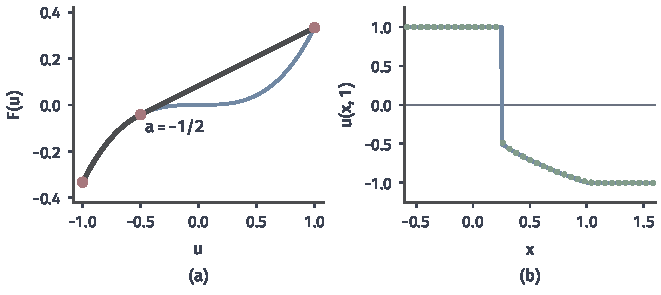
\includegraphics[width=112mm]{figures/06-differential-equations/02-partial-differential-equations/matplotlib/cons-cubic-compound/figure.pdf}
  \caption{非凸通量$F=u^3/3$的Riemann问题$u_l=1$、$u_r=-1$。(a)蓝线是$F$，深灰粗线是上凹包络，红点是端点和切点$a=-1/2$。(b)蓝线是$t=1$的精确解（激波接扇形），绿点是空间步长$2\times10^{-3}$的迎风格式的数值解。}
  \label{fig:cons-cubic-compound}
\end{BookInlineFigure}
